\documentclass{article}

\usepackage{cite}
\usepackage{amsmath,amssymb,amsfonts}
\interdisplaylinepenalty=2500
\usepackage{algorithmic}
\usepackage{graphicx}
\usepackage{textcomp}
\usepackage[table,xcdraw]{xcolor}
\usepackage{cleveref}
\usepackage{pdflscape}
\usepackage{tabularx}
\usepackage{url}
\usepackage{enumitem}
\usepackage{glossaries}
\usepackage{csquotes}
\usepackage{tcolorbox}
\usepackage{caption}
\usepackage{newfloat}
% \usepackage{siunit}

\newcommand\note[1]{\textcolor{gray}{\textit{#1}}}
\newcommand\gibberish[1]{\textcolor{red}{\textit{#1}}}
% \renewcommand\note[1]{}

\makeglossaries
\newglossaryentry{latex}
{
    name=latex,
    description={Is a markup language specially suited 
    for scientific documents}
}

\begin{document}

\title{2D TMD Heterojunction Gas Sensors}
\author{David Freismuth}

\maketitle

\begin{abstract}
Dummy abstract.
\end{abstract}


\section{Introduction}
\label{sec:introduction}
%\note{The importance of gas sensors is made clear. I.e. the need for them in the civil, industrial, medical and military sector. An overview of conventional gas sensors is given. I.e. Bulk-MOX, NDIR, catalytic bead sensor. Novel gas sensors based on 2D structures are presented. Their advantages (small size, flexibility, CMOS-compatibility, sensitivity, specificity) is discussed. Multiple 2D gas sensors are shortly presented. Eventually gas sensors based on 2D TMD heterojunctions are motivated.}

Gas sensing has been used by humans even before the advent of electronic engineering. A prominent example are birds, which accompanied miners in the shafts. If the birds stopped chirping, it was the signal that the oxygen in the air has been replaced by other gases and that the cave should be evacuated as soon as possible \cite{nrc1991}. Since then, gas sensors have evolved drastically, and are now mostly free of any animal cruelty. Today gas sensors are not only used for sensing air quality in underground caves, but are also applied in industrial processes \cite{Johny2016, Wang2017}, in medical fields \cite{Eamsaard2016, Wilson2018}, on military battlefields \cite{Kumar2020a} or are used to sense the gas composition of the environment \cite{Harrou2018}. In the sense of ubiquitous sensing, there is the demand that these sensor become smaller, faster and more power efficient. Trends in that direction allow the development of more efficient industrial processes, increase the efficiency of the medical care or allow precise warnings on the battle field \cite{Wang2022, Kumar2020, Mathew2021}. Market predictions, like the one presented in \cref{fig:gas_sensor_market} confirm this development. \\
\begin{figure}
\centering
    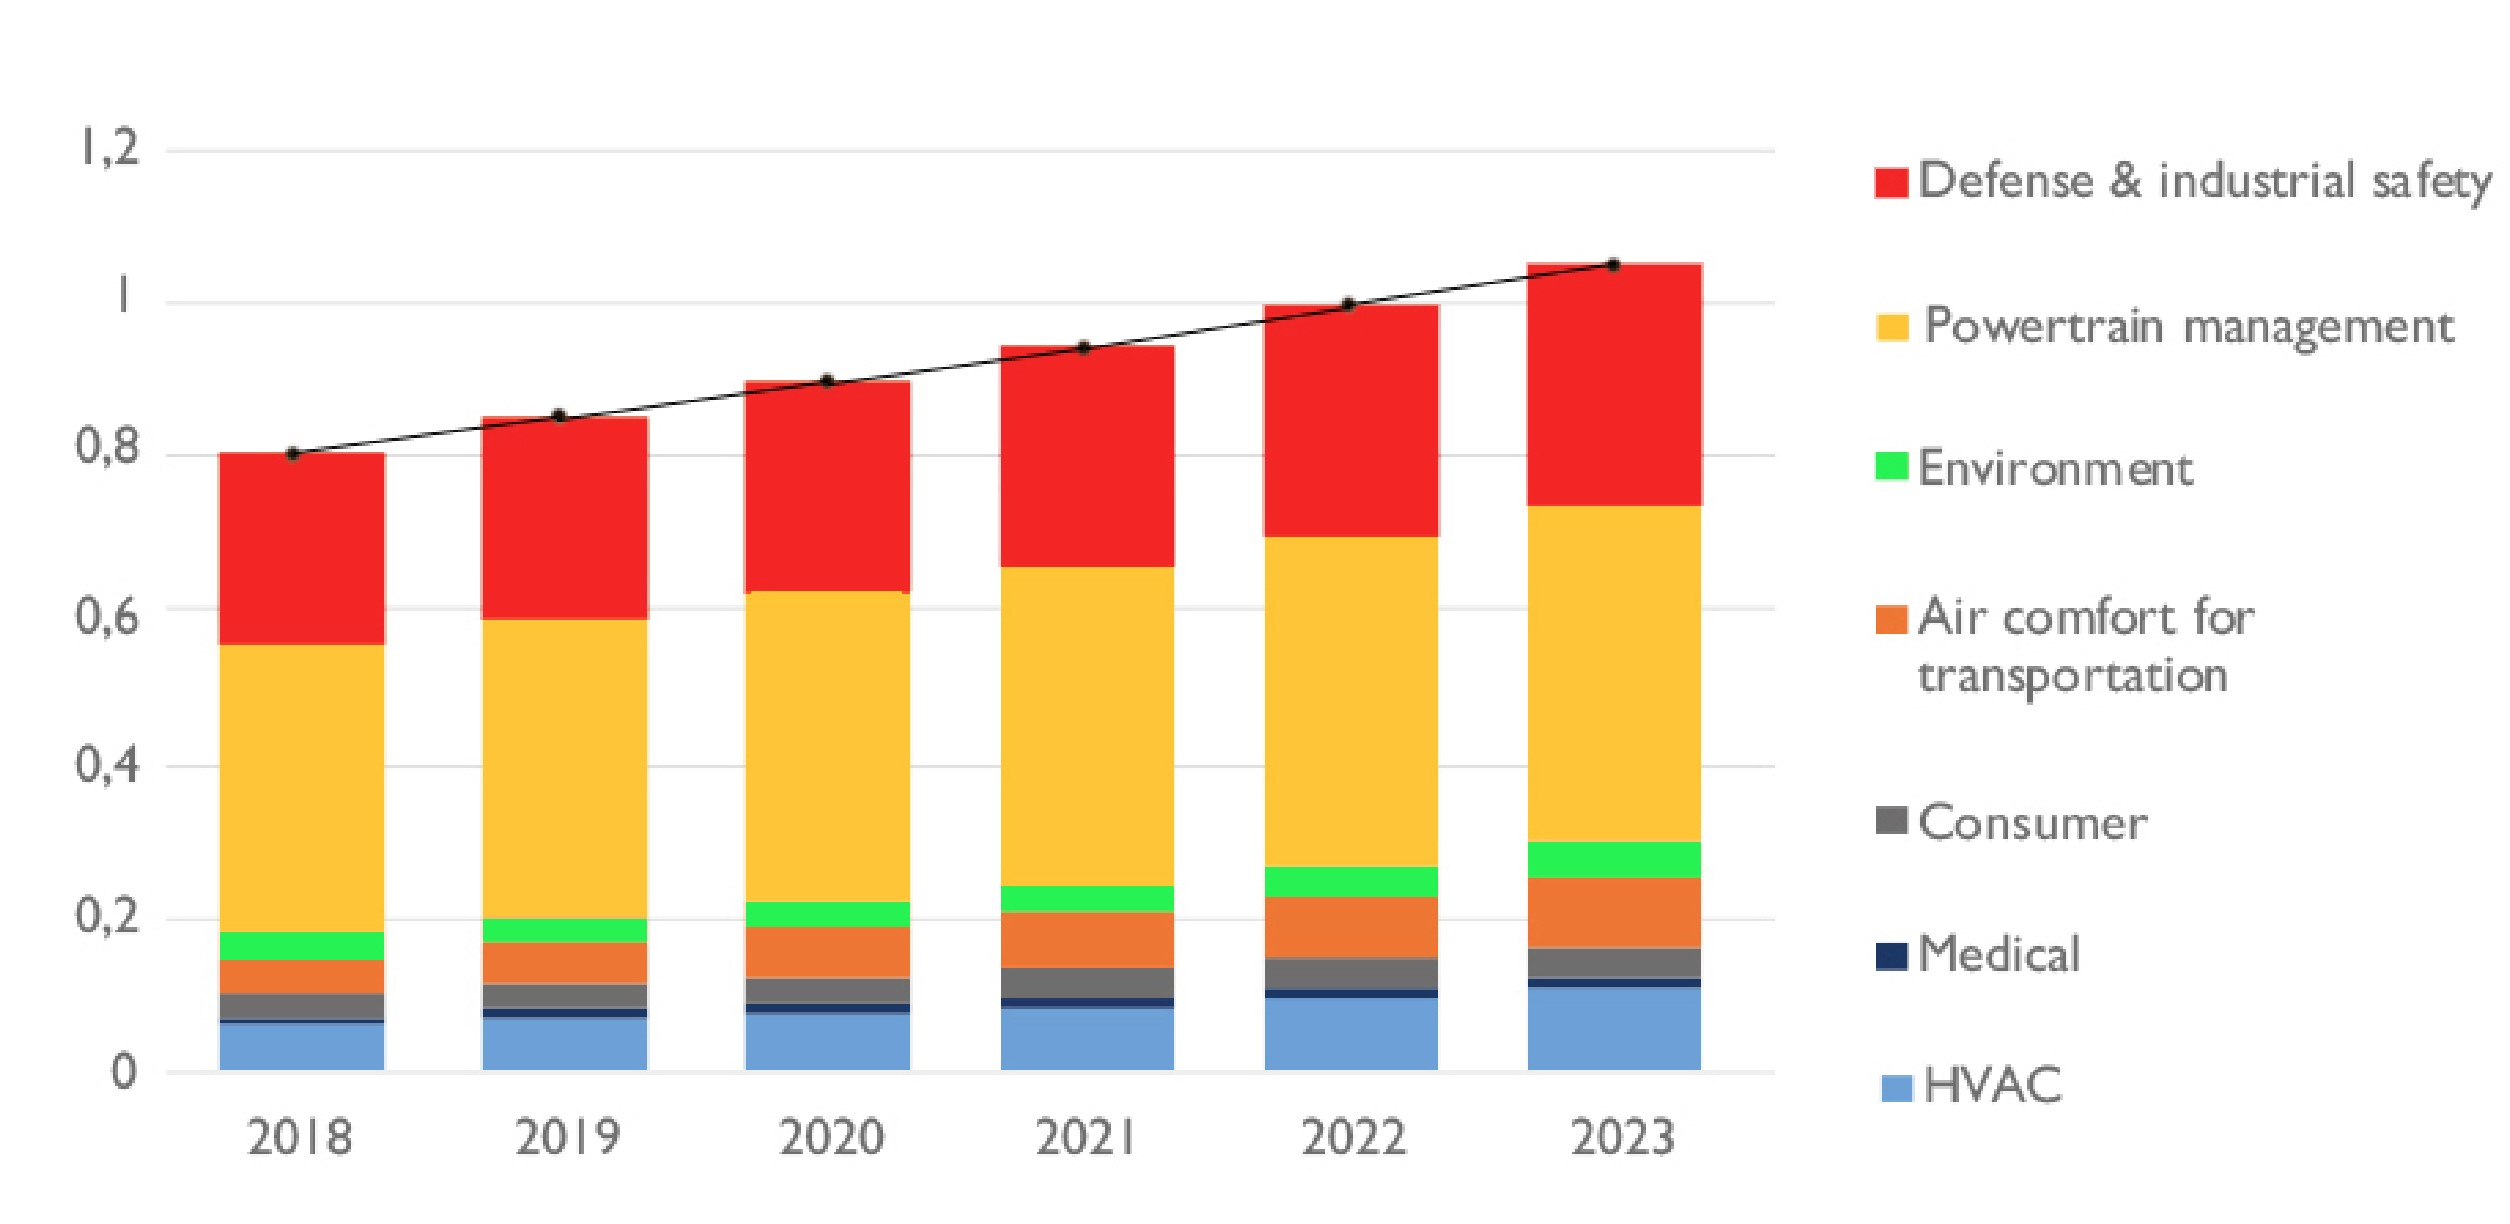
\includegraphics[width=\textwidth]{01_introduction/fig/gas_sensor_market.jpg}
    \caption{The expected market development, as predicted by \cite{yole2021}. Vertical axis is in billion dollars.}
    \label{fig:gas_sensor_market}
\end{figure}
There are a variety of types of gas sensors, whose measurement principles range from optical sensing to chemical effects. One of the most popular gas sensor is the carbon monoxide (CO) sensor, which in many countries is nowadays mandatory to be installed in households \cite{ncsl2018}. The most common version of this sensor is based on a fuel cell like reaction, which generates an electrical current. This current is highly proportional to the CO concentration in the air. This sensor allows detection of concentrations as low as tenths of ppb. First symptoms of carbon monoxide poisoning start at 35 ppm \cite{Goldstein2008}. \\
Another sensor principle relies on the adsorption of the analyte on the surface of a metal oxide bulk structure. The analyte then exchanges electrons with the bulk and modulates its conductivity. This effect serves as metric for the concentration of the analyte in the vicinity of the sensor. The sensor can be made quite small, however it has to heated up to around \SI{400}{\celsius}, so that the adsorption effect takes place. The Taguchi sensor (type TGS 813) \cite{Yamauchi2012, Hartman2021}  is quite popular and its use is very widespread. The Taguchi sensor is sensitive to combustible gases (propan, butan, methan) and can sense concentrations as low as 500 ppm. \\
Another sensor principle is \gls{ndir}. The sensor analyzes the spectrum of light, that is transmitted through the analyte. As most gases have a very specific transmittivity spectrum, and the light spectrum of the source is known, the type and concentration of the analyte gas can be determined. This sensor has the major advantage, that it is able to detect various different gases, where as other sensors are only sensitive to single types of gases. However, the sensor requires long interferometer lengths, and is therefore quite bulky. Such sensor come with a an accuracy of 50 ppm \cite{lp8} (for instance for the gas carbon dioxide). \\
Recent market studies\cite{yole2021, Buckley2020} suggest, that by far the most abundant gas sensor type is the electrochemical one, followed by \gls{ndir} types. The large market shares of these two types can be explained through their good selectivity and relatively low cost. \Cref{fig:gas_sensor_distribution} depicts the relative market revenues, split according to gas sensor type. It can be seen, that 2D materials do not appear in this statistic, which implies that they are not yet feasible for mass market. This paper tries to identify the reasons for that circumstance. \\
\begin{figure}
\centering
    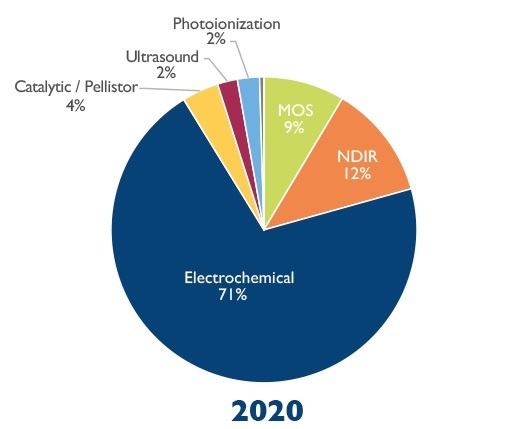
\includegraphics[width=.5\textwidth]{01_introduction/fig/gas_sensor_distribution.jpg}
    \caption{The distribution of gas sensor operating principles \cite{yole2021}.}
    \label{fig:gas_sensor_distribution}
\end{figure}
Great scientific efforts have been undertaken to find new sensing principles that allow further miniaturization and lowering of the power consumption of the sensors. In the last two decades, ample expectations have been made with regards to graphene-based sensors. Scientists believed, that the extreme surface to volume ratio favors a higher sensitivity to gases. Ultimately this assumption could not be satisfied \cite{Geim2013}. One of the major reasons was the lacking band gap of the material. However, progresses in fabrication methods allowed the efficient production of other 2D structures, which exposed the properties, that have been desired from graphene. In \cite{He2012}, one of the first two-dimensional, MoS2 based sensors have been proposed. The device provided a sensitivity of \SI{18}{\percent} at 5 ppm NO2 and a relaxation time of \SI{30}{\minute}. As it was fabricated as a \gls{tft} device on a flexible substrate, it could be bent, without being destroyed. This property enables the integration of the sensor into wearable devices. In \cite{Long2016} a different approach has been followed. A few-layered MoS2 film has been deposited onto a graphene hybrid aerogel scaffold. This device provides a lower detection limit of 50 ppb and a relaxation time of \SI{1}{\minute} (when heated to \SI{200}{\celsius}). \\
These two examples shall testify, that remarkable effects can be shown with 2D structures. One of the most promising material systems is the familiy of \glspl{tmd}. They show strong sensitivity to gas exposure and have an acceptable recovery time. However, one of its most intriguing properties is the potential compatibility to \gls{cmos} fabrication processes. This feature enables the integration of the sensor onto the same silicon wafer as \gls{cmos} transistors. In extension, this implies that the sensor can be integrated onto the same die as its signal conditioning circuits and the digital processing. Effectively, this would cut down on fabrication costs and enable highly integrated gas sensing solutions. Due to these fascinating promises, this publication shall shine a light on gas sensor based on 2D \gls{tmd} structures. \Cref{sec:functionality} explains the workings of 2D \glspl{tmd}. After that, the current fabrication methods are layed out in \cref{sec:fabrication}. In order to give an overview above the tunable parameters of 2D \glspl{tmd}, in \cref{sec:2d_tmd_heterojunction_gas_sensors} two different sensor implementations are compared and discussed. Eventually, a summary and outlook is given in \cref{sec:conclusion}.
\section{Sensor Principle}
\label{sec:functionality}
\note{The operating principles of 2D TMD and 2D TMD heterojunction gas sensors are explained. \\
High surface-to-volume ratio $\rightarrow$ 2D material behaves differently than bulk material (increased reactivity) $\rightarrow$  analyte gas donates/accepts electrons from 2D film $\rightarrow$  carrier density of 2D film is modulated $\rightarrow$  measurable resistance change 
}
\gibberish{
2D \gls{tmd} gas sensor can be categorized as chemiresistors. This means that the electrical resistance of the structure is modulated by the chemical environment of the sensor. Due to the extreme surface to volume ration of these structures, this effect is especially pronounced as the chemical interaction is primarily a surface effect. The resistance modulation effect is based on gas molecules adsorbing onto the surface of the sensor. Depending on the basicity/acidity of the gas, it is donating/accepting electrons from the 2D material. This charge transfer effects the charge density, which, according to equation $a^2 + b^2 = c^2$, affects the conductiviy.  \Cref{fig:sensor_principle} shows a depiction of this behaviour. 
\begin{figure}
    \includegraphics[draft=true]{}
    \caption{Depiction of the sensor principle of 2D \gls{tmd} gas sensors.}
    \label{fig:sensor_principle}
\end{figure}
Sensors that are built like that, exhibit sensitivities of XXX and minimum detection concentrations of YYY. There are multiple techniques that amplify these measures. For instance, targeted pollution of the structure may introduce accumulation points for the analyte, which increases the adsorption rate of the gas and thus the sensitivity of the sensor. Sensors that are modified by targeted inpurities exhibit sensitivities and minimum detection thresholds of XXX and YYY.
Another possibiltiy is to stack the 2D structure vertically with another material. This would create a heterojunction. As \glspl{tmd} are semiconductors, which makes it possible to stack them in a p-n manner, effectively creating a space charge region that further depopulates the device of charge carries. The charge carrier densitiy modulations induced by adsorbed gas therefore creates a greater effect on the conductivity of the sensor. Sensors based on 2D \gls{tmd} heterojunctions reach a sensitivity and minimum detection concentration of XXX and YYY. 
In professor McGonagall's publication it is shown that the sensitivity of 2D \gls{tmd} based gas sensors can be enhanced, when \Gls{uv} light is shone onto the sensor surface. This is due to the tmd molecules that feel more happy when sun light is nearby. The sensor described by McGonagal exhibits a sensitivity and lower detection threshold of XXX and YYY.  
}
\section{Fabrication}
\label{sec:fabrication}
%\note{An overview of the fabrication fo 2D materials is given (\Gls{cvd}, \gls{mbe}, transfer methods). The details of the fabrication of 2D heterojunction devices is given. The heavy dependence of device characteristics to the fabrication method is discussed.}
Fabrication methods include additive and reducing processes. For the extremely thin films, that are required for 2D gas sensors, mostly additive methods are used, as the control of the layer height is much finer. The most prominent 2D film fabrication methods are \gls{mbe}, transfer methods like \gls{dep}, \gls{cvd} and its specialized method \gls{ald}. As the specific fabrication method has major impact on the final sensor performance \cite{Deng2019}, the most important techniques shall be briefly discussed here.
\subsection{Molecular Beam Epitaxy} 
\begin{figure}
    \centering
    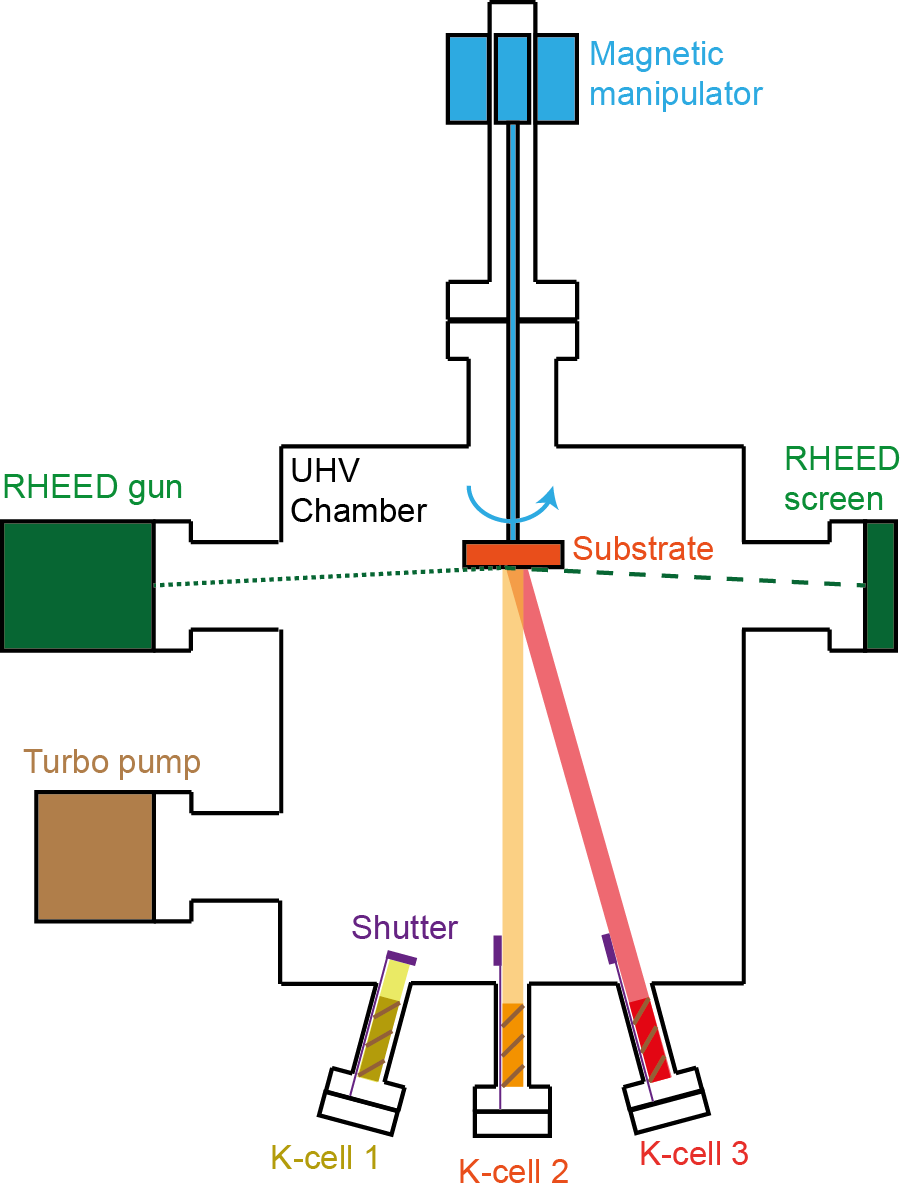
\includegraphics[scale=.7]{03_fabrication/fig/molecular_beam_epitaxy.png}
    \caption{A schematic explaining \gls{mbe}. \cite{Zeljkovic2015}}
    \label{fig:fabrication_mbe}
\end{figure}
\Gls{mbe} is a popular method for growing thin films. Its slow growth rates (ca. \SI{3000}{\nano\meter} per hour) allow fine control over the layer thickness. The principle is based on the target material being evaporated/sublimed in a Knudsen cell. The gas then hits the wafer in the center of the chamber and adsorbs onto the surface. The process is continued until the desired film thickness is reached. This method requires an extremely high vacuum, which makes the process rather expensive, slow, and inflexible.  However, due to the high vacuum and the independence of carrier gases and precursors, \gls{mbe} yields the purest films of all fabrication methods.
\subsection{Dielectrophoresis} 
\begin{figure}
    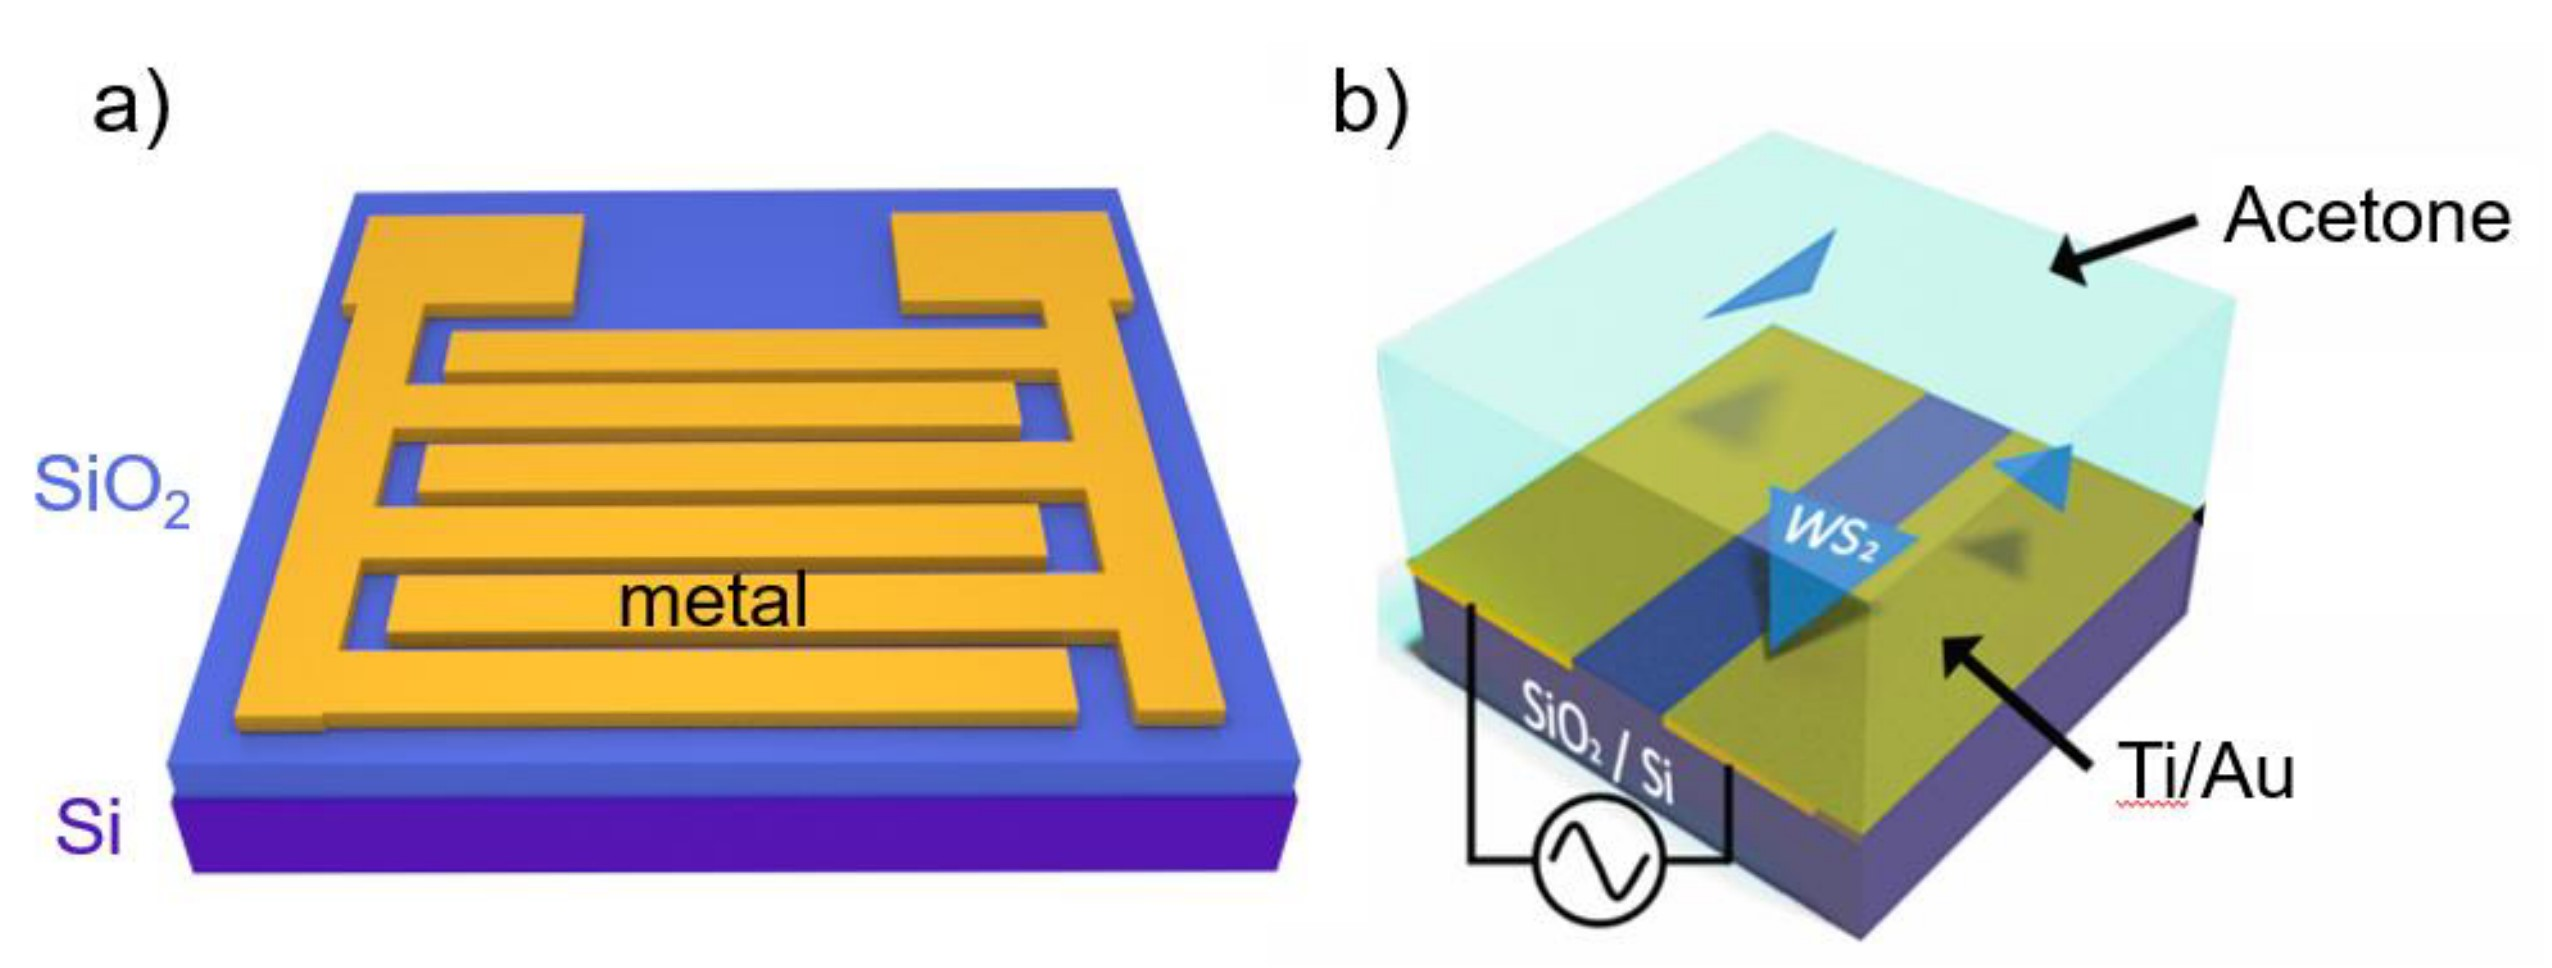
\includegraphics[width=\textwidth]{03_fabrication/fig/dielectrophoresis.jpg}
    \caption{A schematic explaining \gls{dep}. \cite{Deng2019}}
    \label{fig:fabrication_dep}
\end{figure}
Dielectrophoretic assembly utilizes non-uniform electric fields to put pre-fabricated particles to abritrarilly chosen locations. This process is applicable to a wide variety of materials, that do necessarilly have to be dielectric. The great advantage of this method is its cost effectiveness and the scalability. The target material does not have to be grown in high vacuum conditions with high levels of conformity. Rather, flakes of the target material suffice. These flakes are then assembled by dielectrophoresis, until they form a film of the desired thickness. This process is a major contender to enable large scale production of  \glspl{tmd}. The reason why it did not took off yet is that is black magic.
\subsection{Chemical Vapor Deposition}
\begin{figure}
    \includegraphics[draft=true]{}
    \caption{A schematic explaining \gls{cvd}.}
    \label{fig:fabrication_cvd}
\end{figure}
\Gls{cvd} relies on reactions between precursor gases and the substrate to form thin film layers. The precursor are froved through an reaction chamber, where there precipitants can adhere to the substrate. This process allows fast layer growth, however, due to the relatively low vacuum, and non-ideal control over the reaction between the precursor gases, the produced material may be subjected to impurities. 
\subsection{Atomic Layer Deposition}
\begin{figure}
    \includegraphics[draft=true]{}
    \caption{A schematic explaining \gls{ald}.}
    \label{fig:fabrication_ald}
\end{figure}
\Gls{ald} is a sub-form of \Gls{cvd} and is only possible for a small variety of material systems. \Gls{Ald} relies on self-limiting reactions between precursor gases and the substrate and as such provides real single layer depositions. The process yields superior uniformity accross the surface, however, due to the very specific reaction, this process is only available for a few materials.

\section{2D TMD Heterojunction Gas Sensors}
\label{sec:2d_tmd_heterojunction_gas_sensors}
\note{Two 2D TMD heterojunction gas sensors \cite{Kim2020, Liu2021} shall be presented in detail. Their differences in fabrication/performance/scaleability/etc. shall be analyzed. They shall also be compared to conventional gas sensors. Problems that hinder a large scale production shall be identified and possible solution attempts shall be presented.}

\gibberish{As has been stated earlier in this publication, \gls{tmd} gas sensor are very promising in regards to being the next generation of gas sensors. However, there large scale application has yet to be seen. This section shall identify why this is not yet the case. To do that, two gas sensors and their design philosophies shall be shown in detail. Their performance, longevity, scalebality and potential for mass fabrication shall be analyzed and shall be compared to conventional gas sensors.  \\
The first sensor (Sensor 1) is the one proposed by \cite{Kim2020}. It is based on an WSe2/ WS2  heterojunction. The WSe2 film has been exposed to the environment. As it exhibits p-type semiconductor properties, it is especially sensitive to the electron accepting NO2 gas. As explained in \Cref{sec:functionality}, one advantage of heterojunction based gas sensors is the increased sensitivity to gas adsorption. The proposed sensor exhibits another favorable property: A photovoltaic effect. When light of \SI{1000}{\kilo\cd} is shone onto the sensor, a voltage of \SI{5}{\kilo\volt} is generated.  This effect implies, that the sensor does not have to be supplied with an external voltage and that the current, induced by the photovoltaic effect, can be utilized as measurement signal. The layer thickness of both materials was part of a compromise between the magnitude of the photovoltaic effect, and the revovery time of the sensor. A greater layer thickness would increase the photovoltaic effect however, the recovery time of the sensor at room temperature would have been increased. It has been decided to fabricate the sensor with three layers of WSe2 and WS2 respectivelly, resulting in an overall thickness of \SI{4.5}{\nano\meter} (excluding the substrate). The niceness of the layers has been verified via Raman spectroscopy \gls{tem}, \gs{afm} and \gls{eds}. \\
The second sensor (Sensor 2), that shall be discussed, has been fabricated by \cite{Liu2021}. Its strategy is to intentionally pollute MoS2 nanosheets with ZnS in order to generate lots of hetrojunctions, dotted around the surface of the sensor. These impurity sites, for once, create small space charge regions, which modulate the conductivity of the material. Additionally to that, these sites provide docking sites for the analyte gas. This effectivelly increases the adsorption rate of the sensor and thus increases its sensitivity. The sensor does not have photovolotaic properties. The Measurement principle is therefore purely resistive.\\
\subsection{Sensing Performance}
The sensing performance of a gas sensor is usually quantified by its response value $R$. This value is a ratio of its primary measurement parameter in a clean environment and within an environment with specific gas concentration. \Cref{eqn:respone_1,eqn:respone_2,eqn:respone_3} show a few common definitions of the response metric.
\begin{equation}
\label{eqn:respone_1}
    R = \frac{R_a}{R_g}
\end{equation}
\begin{equation}
\label{eqn:respone_2}
    R = \frac{I_a}{I_g}
\end{equation}
\begin{equation}
\label{eqn:respone_3}
    R = \frac{\Delta I_a}{I_g}
\end{equation}
As Sensor 1 relies on current measurement and Sensor 2 on modulation of the conductivity, the response definition from \Cref{eqn:respone_1} and \Cref{eqn:respone_3} shall be used respectivelly. \\ 
Closely related to the response metric of a gas sensor is the lower detection limit $c_{min}$. It specifies the lowest anaylte gas concentration the sensor is able to detect. It is mainly determined by the response and background noise of the sensor. The U.S. Environmental Protection Agency recomands an exposure limit to NO2 of \Si{53}{ppb}. Ideally, the detection limit of gas sensors should be below that value. \\
Another important characteristic is the recovery time $t_r$. It defines how the fast the sensor reacts to changes in gas concentration. Usually it is measured by subjecting the sensor to a specific analyte gas concentration. The recovery time is the time that passes until the sensor reaches \Si{90}{\%} of its final value. \\
\\
Sensor 1 has an response of xxx at a NO2 concentration of XXXppm. Sensor 2 shows a response of YYYppm at the same concentration. The detection limit lies at XXX ppm and yyyppm respectively. Both sensors have been evaluated at room temperature (\SI{25}{\celsius}). The recovery time has been measured to be XXXs and YYYs respectively. 
The quantum nano dot approach of sensor 1 shows that recovery time has been improved significantly. blabla
\begin{table}[]
\centering
\begin{tabular}{lcc}
                    & Sensor 1 & Sensor 2 \\
                    \hline \hline
Response &   1.8 @ \SI{10}{ppm}        &   8.1 @ \SI{10}{ppm}       \\
\hline
Detection Limit    &    N/A      &   \SI{14}{ppb}       \\
\hline
Response Time       &      \SI{6}{\minute}   &  \SI{1}{\minute}        \\
\hline
Recovery Time       &      \SI{12}{\minute}   &  \SI{4.6}{\minute}        \\
\hline
Stability           &      N/A    &   At least \SI{1}{week}       \\
\hline
Working Temperature &      \SI{25}{\celsius}    &  \SI{25}{\celsius} \\
\hline \hline
\end{tabular}
\caption{Comparison between the two presented sensors. All values correspond to NO2 as analyte gas.}
\label{tab:comparison}
\end{table}
\subsection{Fabrication}
Sensor 1 is fabricated by an 6 step process. Starting point is a \Gls{soi} wafer, which has been cleaned with acetone, \gls{ipa} and deionized water.  The WS2 film was deposited by reacting tungsten hexachloride (WCl6) and hydrogen sulfide (H7S) in a \gls{cvd} process. In the same process , WCl6 and Diethylselenide (DESe) has been combined to WSe2. A second substrate has been prepared, where the gold bottom electrode has been prepared. The WS2/WSe2 structure has been transferred onto to gold electrode. Eventually, the palladium top electrode has been patterned onto the WS2/WSe2 structure. \Cref{fig:fabrication_sensor1} depicts this process. The whole process is finished after approx. XXXh and required X tool changes.\\
The fabrication of Sensor 2 starts with the synthesis of the MoS2 nano sheets. For that, a grinding-assisted liquid-phase exfoliation method was used. This method included grinding, disolvation, vigorous sonication and multiple centrifucation steps applied to MoS2 powders. The nanosheets could be obtained from the precipants of that process. The \enquote{pollution} with ZnS has been achieved by mixing the MoS2 nanosheets with Zn(CH3COO)2*2H2O and Na2S*9H20 while being dissolved in deionized water. An interdigitated electrode pair, consisting of Au and Ti, has been prepared on \Gls{SOI}. The prepared MoS2/ZnS solution has then been furhter dilluted with ethanol and subsequently been dripped onto the electrode structure. After a drying step, the MoS2/ZnS structure was finished. The final step consisted of a transfer of the \Gls{SOI} chip onto a copper substrate for better connectivity. It takes approx. YYYh to fabricate this sensor. A total of Y tool transfers were necessary. The whole process is visualized in \Cref{fig:fabrication_sensor2}.
\begin{figure}
\centering
\begin{subfigure}{\textwidth}
    \includegraphics]{}
    \caption{}
    \label{fig:fabrication_sensor1}
\end{subfigure}
\begin{subfigure}{\textwidth}
    \includegraphics]{}
    \caption{}
    \label{fig:fabrication_sensor2}
\end{subfigure}
\caption{The fabrication processes of Sensor 1 (\cref{fig:fabrication_sensor1}) and Sensor 2 \cref{fig:fabrication_sensor2}.}
\label{fig:fabrication}
\end{figure}
\subsection{Scalability}
One of the most important factors that determines the scalability and hence the mass producability of semi conductor devices, is the complexity of their fabrication. With the complexity mostly originating from the count the different fabrication methods being used. Another criteria for good scalability is the compatibility to the \gls{cmos} fabrication process. This property enables the fabrication of the target device on the same wafer as \glspls{mosfet} will be fabricated. This enables the integrated fabrication of sensing device, analog frontend and digital processing without the need of costly transfer processes. Due to its outstanding advantages with regards to footprint size and reduced manufacturing cost, it is a quality that is highly sought after.\\
Fabrication of sensor 1 consists of six steps which are mainly executable within a \gls{cvd} chamber. A single transfer process is necessary, in order to transport the 2D material onto the contact electrodes. Apart from the transfer step, the process is simple and shows potential for scaling. Compaitiblity to \gls{cmos} processes has to be judged on a per-case basis, as a temperature of \SI{700}{\celsius} is necessary, during the film synthesis. This temperature could reactivate the diffusion in some doped regions and therefore could be detrimental to the integration into \gls{cmos} processes.\\
Sensor 2 fabrication is concluded after seven steps. Although, the transfer process uses \gls{dep}, and as such could have potential to be scalable, the fabrication of the nanosheets and the application of the nano dots, is a highly manual process, which seems to be hardly automatable. As no high temperature processes are needed, \gls{cmos} compatibility is given. The only challenge is to introduce the dissolved nanoparticles into the fabrication line.
\subsection{Stability}
The stability (or life span) specifies the period of time, the sensor adheres to its specification. a high stability decreases the rate at which sensors have to be replaced. Usually the readout of the sensors is also simplified, as fewer drift compensation has to be considered. The life span of a sensor is highly dependent on its environment. For instance, the commercially available NO2 sensor FECS42-20 specifies a life span of over two years \cite{Figaro}. \\ 
Sensor 1 did not provide any measures on long term drift of the sensor parameters. There seem to be no other publications with identical layer stack configuration. The closest device, sensor 1 could compare to, is the one presented in \cite{Wu2020} as both sensors expose a WSe2 surface to the environment. There, no significant degradation has been noticed, within the test period of 60 days. \\
An evaluation of the long term stability of sensor 2 has been done. The response metric dropped from 7.3 to 7.1 within one week and seemed to stabilize there.
}
\section{Conclusion}
\label{sec:conclusion}
%\note{The delivered information is shortly reiterated. Current problems of 2D TMD heterojunction gas sensors are stated and possible solutions are presented. An outlook to future developments is given.}

An overview of the measuring principle and fabrication of conventional and state of the art gas sensors has been given. The advantages and shortcomings of gas sensors, based on 2D materials have been identified and discussed. By comparing two different 2D gas sensors, it has been made clear, that such sensors can not yet compete with commercially available ones. Although superior response values, response times and selectivities can be achived, such sensor often lack in stability, and loose their favorable properties after a few weeks, due to the degradation of the sensor surface. Another steep challenge is the commercialization of such sensors. To achieve financial viability, the fabrication of such sensors has to move from laboratories to semiconductor foundries, in order to scale up the fabricated quantities. This requires the fabrication process to be mundane enough, to comply to the fabrication processes of these foundries. The two presented sensors show potential on being compatible for mass production, which exemplifies that formidable gas sensing characteristics can be achieved, without usage of exotic materials and fabrication processes. Upcoming research has to focus on stabilization of such sensors and on the integration into \gls{cmos} processes. If that is mastered, highly integrateable gas sensors with included digital processing are possible.


\bibliographystyle{ieeetr}
\bibliography{lib/emerging_devices}
\printglossaries


\end{document}
